\documentclass{beamer}
\usepackage[utf8]{inputenc}
\usepackage[UKenglish]{babel}
\usepackage[UKenglish]{isodate}
\usepackage{amsmath}
\usepackage{mathtools}
\usepackage{tikz}
\usepackage{complexity}

\usetikzlibrary{shapes}
\usetikzlibrary{arrows}
\usetikzlibrary{arrows.meta}
\usetikzlibrary{positioning}
\usetikzlibrary{overlay-beamer-styles}
\usetikzlibrary{shapes.callouts}
\usetikzlibrary{cd}

\beamertemplatenavigationsymbolsempty
\usetheme{metropolis}
\setbeamercolor{background canvas}{bg=white}
%\usecolortheme{rose}

\definecolor{color1}{HTML}{1B9E77}
\definecolor{color2}{HTML}{D95F02}

\newcommand{\WMC}{\textup{WMC}}
\newcommand{\WFOMC}{\textup{(W)FOMC}}
\newcommand{\WMI}{\textup{WMI}}
\newcommand{\WFOMI}{\textup{WFOMI}}
\newcommand{\AMC}{\textup{AMC}}
\newcommand{\pbp}{\textup{PBP}}
\newcommand{\SPPP}{\textup{SP}}

\DeclareMathOperator{\MC}{MC}

\begin{document}
\addtobeamertemplate{block begin}{\setlength\abovedisplayskip{0pt}}

\begin{frame}{A Slightly Different Setup}
  \begin{itemize}
    \item A \alert{theory} is a conjunction of clauses
    \item A \alert{clause} is a sentence in many-sorted function-free first-order logic with equality
    \item No restrictions on the number of variables
    \item Constants are allowed
    \item Skolemization eliminates existential quantifiers
  \end{itemize}
  \begin{example}[Injective functions]
    \begin{gather*}
      (\forall x \in \Delta\text{. }\forall y, z \in \Gamma\text{. } P(x, y) \land P(x, z) \to y = z) \land \\
      (\forall x \in \Delta\text{. }\exists y \in \Gamma\text{. } P(x, y)) \land \\
      (\forall w, x \in \Delta\text{. }\forall y \in \Gamma\text{. } P(w, y) \land P(x, y) \to w = x)
    \end{gather*}
  \end{example}
\end{frame}

\begin{frame}{Compilation Rules}
  \begin{example}[Independence]
    Input formula:
    \begin{gather}
      ({\color{color1} \forall x, y \in \Omega\text{. }x=y}) \land \label{eq:1} \tag{{\color{color1} 1}} \\
      ({\color{color2} \forall x \in \Delta\text{. }\forall y, z \in \Gamma\text{. }P(x, y) \land P(x, z) \to y=z}) \land \label{eq:2} \tag{{\color{color2} 2}} \\
      ({\color{color2} \forall w, x \in \Delta\text{. }\forall y \in \Gamma\text{. }P(w, y) \land P(x, y) \to w=x}) \label{eq:3} \tag{{\color{color2} 3}}
    \end{gather}
    \pause
    \[
      G =
      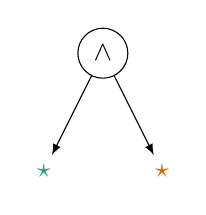
\begin{tikzpicture}[edge from parent/.style={draw,-latex},baseline=(current bounding box.center)]
        \node[draw,circle] {$\land$}
        child {node {\color{color1} $\star$}}
        child {node {\color{color2} $\star$}}
        ;
      \end{tikzpicture},
      \qquad
      L = \langle {\color{color1} \eqref{eq:1}}, {\color{color2} \eqref{eq:2} \land \eqref{eq:3}} \rangle
    \]
  \end{example}
\end{frame}
% stars mark edges to nowhere and they are associated with the formulas in L via a certain order

\begin{frame}{The Algebraic Interpretation}
  \begin{columns}
    \begin{column}{0.25\textwidth}
      \centering
      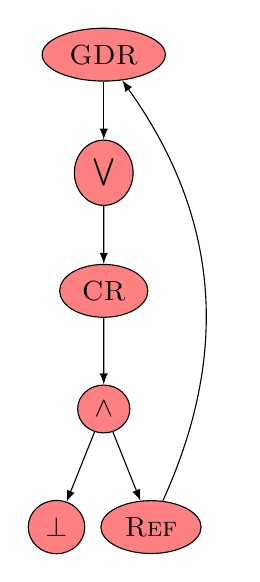
\begin{tikzpicture}[every node/.style={draw,ellipse},edge from parent/.style={draw,-latex},sibling distance=12mm,level distance=15mm]
        \node[fill=red!50,fill on=<2>] (dr) {\textsc{GDR}}
        child {node[fill=red!50,fill on=<3>] {$\bigvee$}
                child {node[fill=red!50, fill on=<4>] {\textsc{CR}}
                  child {node[fill=red!50, fill on=<5>] {$\land$}
                    child {node[fill=red!50, fill on=<6>] {$\bot$}}
                    child {node[fill=red!50, fill on=<7>] (ref) {\textsc{Ref}}}
        }}};
        \draw[-latex, bend right] (ref) to (dr);
      \end{tikzpicture}
    \end{column}
    \begin{column}{0.75\textwidth}
      \begin{align*}
        f(m, n) &= \onslide<3->{\sum_{l=0}^m \binom{m}{l}} \onslide<6->{[l<2]} \onslide<5->{\times} \onslide<7->{f(m-l, n-1)}\\
        \onslide<8>{&= f(m, n-1) + mf(m-1, n-1)}
      \end{align*}
      \onslide<6>{
        \[
          [\phi] =
          \begin{cases}
            1 & \text{if } \phi \\
            0 & \text{if } \neg\phi
          \end{cases}
          \]
      }
    \end{column}
  \end{columns}
\end{frame}

\begin{frame}{Workflow}
  \begin{block}{with \textsc{ForcLift}}
    \begin{enumerate}
      \item Compile the formula to a \alert{circuit}
      \item Evaluate to get the answer
    \end{enumerate}
  \end{block}
  \begin{block}{with \textsc{Crane} (my work)}
    \begin{enumerate}
      \item Compile the formula to a \alert{graph}
      \item Extract the definitions of functions
      \item Simplify
      \item Supplement with \alert{base cases}
      \item Evaluate to get the answer
    \end{enumerate}
  \end{block}
\end{frame}

% \begin{frame}{More Formally\ldots}
%   \begin{definition}
%     A \alert{first-order deterministic decomposable negation normal form computational graph} (FCG) is a
%     \begin{itemize}
%     \item directed graph
%     \item (which is weakly connected)
%     \item with a single source,
%     \item labelled vertices,
%     \item and ordered outgoing edges.
%     \end{itemize}
%   \end{definition}
% \end{frame}

%% \begin{frame}{Compilation as Search}
%%   \begin{definition}
%%     A \alert{(search) state} is a tuple \structure{$(G, C, L)$}, where:
%%     \begin{itemize}
%%     \item \structure{$G$} is an FCG (or \texttt{null}),
%%     \item \structure{$C$} is a compilation cache that maps integers to sets of pairs $(\phi, v)$, where $\phi$ is a formula, and $v$ is a vertex of $G$ (which is used to identify opportunities for recursion),
%%     \item and \structure{$L$} is a list of formulas (that are yet to be compiled). (Note that the order is crucial!)
%%     \end{itemize}
%%   \end{definition}
%%   The search algorithm combines greedy and breadth-first search:
%% \end{frame}

\begin{frame}{Major Directions for Future Work}
  \begin{itemize}
    \item An algebraic description of what kind of sequences and functions with
          domain $\mathbb{N}_{0}^{k}$ are computable in this way
          \begin{itemize}
            \item monotonicity, maximal growth rate, etc.
          \end{itemize}
    \item A different input format or logic that allows the same approach to
          capture more computations
          \begin{itemize}
            \item fixed-point logic with counting
            \item `let domain $\Delta \coloneqq \{\, 1, 2, \dots, \MC(\phi) \,\}$'
          \end{itemize}
    \item parameterised Markov logic networks
    \begin{itemize}
      \item `What equations do the domain sizes have to satisfy for the
            probability of event $E$ to be at least $95\%$?'
    \end{itemize}
  \end{itemize}
\end{frame}

\end{document}
